\documentclass{beamer}
%\usepackage[T1]{fontenc}
\usepackage[utf8]{inputenc}
%\usepackage{lmodern}  % Use the Latin Modern font family

\usepackage{latexsym,amsmath,xcolor,bm, amssymb, color, tikz, graphicx, amsthm, mathtools}
\usepackage{algorithm}
\usepackage{algorithmic}
\usepackage{hyperref}
\usepackage{float}     
\usepackage{CJKutf8}
\usepackage{multicol}

\DeclareMathOperator*{\argmax}{arg\,max}
\DeclareMathOperator*{\argmin}{arg\,min}
\DeclareMathOperator{\sign}{sign}
\DeclareMathOperator{\Tr}{Tr}

\makeatletter
\DeclareRobustCommand\onedot{\futurelet\@let@token\@onedot}
\def\@onedot{\ifx\@let@token.\else.\null\fi\xspace}
\def\eg{\emph{e.g}\onedot} 
\def\Eg{\emph{E.g}\onedot}
\def\ie{\emph{i.e}\onedot} 
\def\Ie{\emph{I.e}\onedot}
\def\cf{\emph{c.f}\onedot} 
\def\Cf{\emph{C.f}\onedot}
\def\etc{\emph{etc}\onedot} 
\def\vs{\emph{vs}\onedot}
\def\wrt{w.r.t\onedot} 
\def\dof{d.o.f\onedot}
\def\etal{\emph{et al}\onedot}
\makeatother


\usetheme{Madrid}
\useinnertheme{circles}


\definecolor{ColorUNR}{HTML}{0b2755} 
\usecolortheme[named=ColorUNR]{structure}
%\usecolortheme[named=ColorUNR]{exampleblock}

%\setbeamertemplate{blocks}[rounded][shadow=true]
%\setbeamercolor{block body}{fg=black,bg=white}



%------------------------------------------------------------
%This block of code defines the information to appear in the
%Title page
\title %optional
{Cierre Training Camp 2025}

\subtitle{Ceremonia de Clausura}

%\subtitle{with applications to persuation and lie production}
% \author % (optional)
% {Author Name}

\author[Matias Ramos]{Matias Ramos}

\institute[]{Universidad Tecnológica Nacional - Facultad Regional Santa Fe}
\date[TC 2025]{Training Camp 2025}
\titlegraphic{\includegraphics[clip,height=2cm,keepaspectratio]{logos/tcarg.jpeg}}

%End of title page configuration block
%------------------------------------------------------------


%------------------------------------------------------------
%The next block of commands puts the table of contents at the 
%beginning of each section and highlights the current section:
\AtBeginSection[]
{
  \begin{frame}
    \frametitle{Outline}
    \tableofcontents[currentsection]
  \end{frame}
}
%------------------------------------------------------------


\begin{document}


%The next statement creates the title page.
\frame{\titlepage}


%------------------------------------------------------------
% Frame de Sponsors, me parece mejor ponerlo al principio
% Antes del índice/contenido

% --- Sponsors Frame 1: Organizador & Diamond Plus ---


% First sponsors frame: Organizador and Diamond Plus
\begin{frame}{Gracias Sponsors!}
    \begin{columns}[t]
        \column{0.5\textwidth}
        \centering
        Organizador\\
        \vspace{0.5cm}
        \includegraphics[width=1\textwidth,keepaspectratio]{logos/aapc.png}
        \includegraphics[width=1\textwidth,keepaspectratio]{logos/utn_santafe.png}
        \column{0.5\textwidth}
        \centering
        Diamond Plus\\
        \includegraphics[width=1\textwidth,keepaspectratio]{logos/GTSlogo.jpeg}
    \end{columns}
\end{frame}

% --- Sponsors Frame 2: Gold & Oro ---

\begin{frame}{Gracias Sponsors!}
    % Platino at the top, full width
    \centering
    Platino\\
    \includegraphics[width=0.6\textwidth,keepaspectratio]{logos/folder.png}
    
    \vfill
    
    % Gold and Oro at the bottom in two columns
    \begin{columns}[b]
        % Gold column
        \column{0.5\textwidth}
        \centering
        Gold\\
        \includegraphics[width=0.8\textwidth,keepaspectratio]{logos/neuralsoft.png}
        % Oro column
        \column{0.5\textwidth}
            \centering
        Oro\\
        \includegraphics[width=0.8\textwidth,keepaspectratio]{logos/jerarquicos.jpg}
    \end{columns}
\end{frame}

% --- Sponsors Frame 3: Aliado ---

\begin{frame}{Gracias Sponsors!}
    \centering
    Aliado\\
    \vspace{1cm}
    \includegraphics[width=0.6\textwidth,keepaspectratio]{logos/santa_fe_logo_v2.jpg}
\end{frame}


\section{Gracias por venir}

\begin{frame}{Gracias por venir}
\begin{center}
\Large
¡Muchas gracias por participar en el Training Camp 2025!

\vspace{1cm}

Esperamos que hayan disfrutado de esta experiencia y que hayan aprendido mucho.

\vspace{1cm}

¡Nos vemos en la próxima edición!
\end{center}
\end{frame}

\begin{frame}{Participantes por País}
\begin{center}
\Large
\textbf{¡168 participantes presentes!}

\vspace{0.5cm}

\normalsize
\textbf{Distribución por países:}

\vspace{0.3cm}

\begin{itemize}
\item \textbf{Argentina:} 117 participantes
\item \textbf{Perú:} 14 participantes  
\item \textbf{Chile:} 13 participantes
\item \textbf{Costa Rica:} 8 participantes
\item \textbf{Colombia:} 7 participantes
\item \textbf{México:} 5 participantes
\item \textbf{Uruguay:} 3 participantes
\item \textbf{Brasil:} 1 participante
\end{itemize}

\vspace{0.5cm}

\textbf{¡Gracias por hacer de este evento un éxito internacional!}
\end{center}
\end{frame}

\begin{frame}{Diversidad Regional}
\begin{center}
\Large
\textbf{8 países representados}

\vspace{0.5cm}

% --- Dots Only: Geographically Accurate and All Visible ---

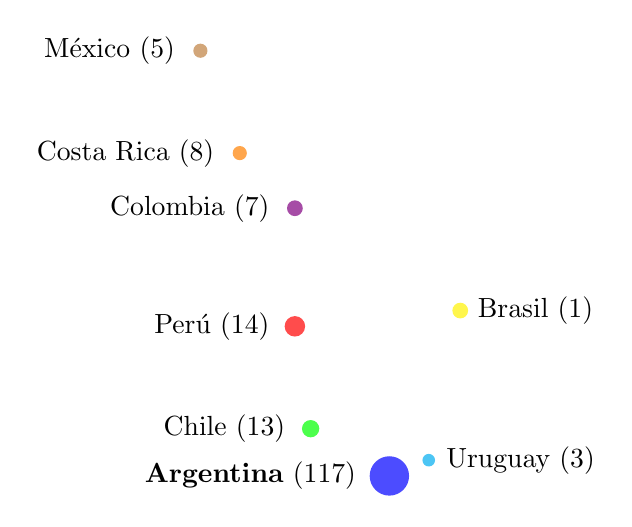
\begin{tikzpicture}[scale=1.0]
  % Argentina
  \fill[blue,opacity=0.7] (3.2,1.1) circle (0.25); % 117
  \node[left] at (2.9,1.1) {\textbf{Argentina} (117)};
  % Uruguay
  \fill[cyan,opacity=0.7] (3.7,1.3) circle (0.08); % 3
  \node[right] at (3.8,1.3) {Uruguay (3)};
  % Chile
  \fill[green,opacity=0.7] (2.2,1.7) circle (0.11); % 13
  \node[left] at (2.0,1.7) {Chile (13)};
  % Peru
  \fill[red,opacity=0.7] (2.0,3.0) circle (0.13); % 14
  \node[left] at (1.8,3.0) {Perú (14)};
  % Colombia
  \fill[violet,opacity=0.7] (2.0,4.5) circle (0.10); % 7
  \node[left] at (1.8,4.5) {Colombia (7)};
  % Costa Rica
  \fill[orange,opacity=0.7] (1.3,5.2) circle (0.09); % 8
  \node[left] at (1.1,5.2) {Costa Rica (8)};
  % Mexico
  \fill[brown,opacity=0.7] (0.8,6.5) circle (0.09); % 5
  \node[left] at (0.6,6.5) {México (5)};
  % Brasil
  \fill[yellow,opacity=0.7] (4.1,3.2) circle (0.10); % 1 (make visible)
  \node[right] at (4.2,3.2) {Brasil (1)};
\end{tikzpicture}

\vspace{0.5cm}

\textbf{América Latina unida por la programación competitiva}

\vspace{0.3cm}

\normalsize
¡Cada país aportó su talento y entusiasmo!

\vspace{0.2cm}

\textbf{Argentina lidera con el 70\% de los participantes}
\end{center}
\end{frame}


\section{Entrenaron una banda}

\begin{frame}{Entrenaron una banda}
\begin{center}
\Large
¡Felicitaciones a todos los participantes!

\vspace{1cm}

Han completado exitosamente el Training Camp 2025

\vspace{1cm}

Cada uno de ustedes ha demostrado dedicación, esfuerzo y pasión por la programación competitiva.

\vspace{1cm}

¡Son una banda increíble!
\end{center}
\end{frame}


\section{y ahora... los premios}

\begin{frame}{Vino mucha gente de Tucumán}
\begin{center}
\Large
\textbf{¡Vino mucha gente de Tucumán!}

\vspace{1cm}

\fcolorbox{blue}{blue}{\includegraphics[width=0.4\textwidth,keepaspectratio]{logos/unt_logo.png}}

\vspace{1cm}

\normalsize
\textbf{Universidad Nacional de Tucumán}

\vspace{0.5cm}

¡Gracias por su participación!
\end{center}
\end{frame}

\begin{frame}{SPOILER ALERT}
\begin{center}
\Huge
\textbf{SPOILER ALERT}

\vspace{2cm}

\Large
¡Algo importante está por venir!
\end{center}
\end{frame}

\begin{frame}{TC 2026?}
\begin{center}
\includegraphics[width=0.98\textwidth,height=0.9\textheight,keepaspectratio]{img/tucu.jpeg}
\end{center}
\end{frame}

\begin{frame}{y ahora... los premios}
\begin{center}
\Large
¡Es momento de reconocer a los mejores!

\vspace{1cm}

Los participantes que se destacaron durante el Training Camp 2025

\vspace{1cm}

Recibirán sus merecidos premios y reconocimientos.

\vspace{1cm}

¡Aplausos para todos los ganadores!
\end{center}
\end{frame}


\section{y que hago con todo lo que aprendi?}

\begin{frame}{y que hago con todo lo que aprendi?}
\begin{center}
\Large
¡Aplica todo lo que aprendiste!

\vspace{1cm}

\begin{itemize}
\item Participa en competencias de programación
\item Practica en plataformas online
\item Comparte conocimiento con otros
\item Sigue aprendiendo y mejorando
\end{itemize}

\vspace{1cm}

¡El conocimiento se multiplica cuando se comparte!
\end{center}
\end{frame}

\begin{frame}{Maratona Feminina de Programação (MFP) - Información General}
\begin{center}
\includegraphics[width=0.2\textwidth,keepaspectratio]{img/mfp_logo.jpeg}

\vspace{0.3cm}

\Large
\textbf{Maratona Feminina de Programação}

\vspace{0.2cm}

\normalsize
\textbf{Competencia exclusiva para mujeres en programación}

\vspace{0.3cm}

\begin{itemize}
\item \textbf{Objetivo:} Promover la participación femenina en programación competitiva
\item \textbf{Formato:} Competencia individual o en equipos
\item \textbf{Duración:} 5 horas de competencia intensiva
\item \textbf{Lenguajes:} C/C++, Python, Java, entre otros
\item \textbf{Organización:} Sociedad Brasileña de Computación (SBC)
\end{itemize}

\vspace{0.3cm}

\textbf{¡Una oportunidad única para demostrar tu talento!}

\vspace{0.2cm}

\small
\url{https://www.instagram.com/mfp.sbc}
\end{center}
\end{frame}

\begin{frame}{Maratona Feminina de Programação (MFP) - Beneficios y Participación}
\begin{center}
\Large
\textbf{¿Por qué participar en MFP?}

\vspace{0.3cm}

\normalsize
\begin{itemize}
\item \textbf{Networking:} Conoce a otras programadoras apasionadas
\item \textbf{Desarrollo:} Mejora tus habilidades de resolución de problemas
\item \textbf{Visibilidad:} Demuestra tu talento en la comunidad
\item \textbf{Mentoría:} Acceso a mentoras experimentadas
\item \textbf{Oportunidades:} Puertas abiertas a competencias internacionales
\end{itemize}

\vspace{0.3cm}

\textbf{¡Rompe barreras y construye tu futuro en tecnología!}

\vspace{0.2cm}

\normalsize
\textbf{Próxima edición:} Consulta las fechas en sus redes sociales

\vspace{0.1cm}

\small
\url{https://www.instagram.com/mfp.sbc}
\end{center}
\end{frame}

\begin{frame}{Torneo Argentino de Programación (TAP) - Información General}
\begin{center}
\includegraphics[width=0.2\textwidth,keepaspectratio]{img/tap_logo.png}

\vspace{0.3cm}

\Large
\textbf{15º Torneo Argentino de Programación 2025}

\vspace{0.2cm}

\normalsize
\textbf{Sábado 23 de agosto de 2025}

\vspace{0.2cm}

\begin{itemize}
\item \textbf{Competencia:} 5 horas de duración
\item \textbf{Equipos:} 3 personas por equipo (1 PC)
\item \textbf{Lenguajes:} C/C++, Python, Java o Kotlin
\item \textbf{Requisito:} Ser estudiante de educación superior en Argentina
\item \textbf{Clasificación:} Para ICPC Latinoamérica (Chile 2026)
\end{itemize}

\vspace{0.2cm}

\textbf{¡Inscripción hasta el 20 de agosto!}

\vspace{0.1cm}

\small
\url{https://icpc.global/regionals/finder/TAP-2026}
\end{center}
\end{frame}

\begin{frame}{Torneo Argentino de Programación (TAP) - Sedes de Competencia}
\begin{center}
\Large
\textbf{Sedes de Competencia 2025}

\vspace{0.3cm}

\normalsize
\begin{columns}[t]
\column{0.5\textwidth}
\begin{itemize}
\item \textbf{UNJu} (Jujuy)
\item \textbf{UNSa} (Nueva Orán, Salta)
\item \textbf{UNT} (Tucumán)
\item \textbf{UNdeC} (La Rioja)
\item \textbf{FAMAF-UNC} (Córdoba)
\item \textbf{UNRC} (Córdoba)
\item \textbf{UTN Santa Fe}
\end{itemize}

\column{0.5\textwidth}
\begin{itemize}
\item \textbf{UNLAM} (Bs. As.)
\item \textbf{UNLP} (Bs. As.)
\item \textbf{Inst. Balseiro} (Río Negro)
\item \textbf{UTN Resistencia} \textbf{¡Nueva sede!}
\end{itemize}

\end{columns}

\vspace{0.3cm}

\textbf{¡Tu universidad puede ser sede!}

\vspace{0.2cm}

\normalsize
Solo necesitás conexión a internet

\vspace{0.2cm}

\small
\url{https://icpc.com.ar/tap}
\end{center}
\end{frame}

\begin{frame}{Regional Sudamérica-Sur}
\begin{center}
\includegraphics[width=0.3\textwidth,keepaspectratio]{img/regional_logo.jpg}

\vspace{0.3cm}

\Large
\textbf{Regional Sudamérica-Sur 2025}

\vspace{0.2cm}

\normalsize
\textbf{8 de noviembre de 2025}

\vspace{0.2cm}

\begin{itemize}
\item \textbf{Participantes:} Equipos clasificados del TAP y otros países
\item \textbf{Países:} Argentina, Chile, Uruguay, Paraguay, Bolivia
\item \textbf{Formato:} 5 horas de competencia intensiva
\item \textbf{Premio:} Clasificación a PDA 2026
\end{itemize}

\vspace{0.2cm}

\textbf{¡El siguiente paso después del TAP!}

\vspace{0.1cm}

\small
\url{https://icpc.com.ar/regional-latinoamericana}
\end{center}
\end{frame}

\begin{frame}{Programadores de América 2026}
\begin{center}
\Large
\textbf{Programadores de América 2026}

\vspace{0.3cm}

\normalsize
\textbf{Santiago de Chile, Marzo 2026}

\vspace{0.3cm}

\begin{columns}[t]
\column{0.5\textwidth}
\centering
\textbf{Pontificia Universidad}\\
\textbf{Católica de Chile}

\vspace{0.5cm}

\textbf{Universidad organizadora}

\column{0.5\textwidth}
\centering
\textbf{Universidad Técnica}\\
\textbf{Federico Santa María}

\vspace{0.5cm}

\textbf{Universidad co-organizadora}

\end{columns}

\vspace{0.5cm}

\begin{itemize}
\item \textbf{Competencia:} Final continental de programación
\item \textbf{Participantes:} Mejores equipos de Latinoamérica
\item \textbf{Formato:} 5 horas de competencia intensiva
\item \textbf{Premio:} Clasificación a la Final Mundial ICPC 2026
\end{itemize}

\vspace{0.3cm}

\textbf{¡La meta final de todo programador competitivo!}

\vspace{0.1cm}

\small
\url{https://icpc.global}
\end{center}
\end{frame}


\section{Gracias a todos}

\begin{frame}{Gracias a todos}
\begin{center}
\Large
¡Gracias a todos por hacer posible el Training Camp 2025!

\vspace{1cm}

\begin{itemize}
\item A los participantes por su entusiasmo y dedicación
\item A los sponsors por su apoyo incondicional
\item A los organizadores por su trabajo incansable
\item A la comunidad por su colaboración
\end{itemize}

\vspace{1cm}

¡Sin ustedes esto no hubiera sido posible!

\vspace{1cm}

¡Hasta la próxima edición!
\end{center}
\end{frame}

\end{document}